%<dscrpt>Autour des trisectrices : théorème de Morley, cardioïdes.</dscrpt>
L'objet de ce probl{\`e}me est de pr{\'e}senter quelques r{\'e}sultats relatifs aux trisectrices d'un angle. Les
trisectrices sont les droites qui d{\'e}coupent un angle en trois angles {\'e}gaux. On d{\'e}montrera le th{\'e}or{\`e}me de Morley (fig \ref{fig:Etrisec_1}) et une propri{\'e}t{\'e} des cardio{\"\i}des (fig \ref{fig:Etrisec_2}).

\begin{figure}[ht]
  \centering
  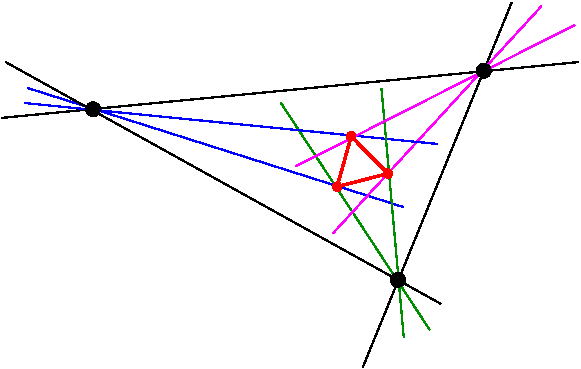
\includegraphics{Etrisec_1.pdf}
  \caption{Th{\'e}or{\`e}me de Morley}
  \label{fig:Etrisec_1}
\end{figure}

Dans tout le probl{\`e}me, le plan est muni d'un rep{\`e}re orthonorm{\'e} direct qui permet de d{\'e}finir l'affixe complexe d'un point et le repr{\'e}sentant d'un nombre complexe.\newline
On utilisera tr{\`e}s souvent la relation $1+j+j^2=0$ avec $j=e^{\frac{2i\pi}{3}}$
\begin{itemize}
\item Les nombres complexes $a$, $b$, $c$ sont les affixes de trois
points $A$, $B$, $C$.

\item Les nombres r{\'e}els $\alpha$, $\beta$, $\gamma$ sont dans
$]0,\frac{\pi}{3}[$ et v{\'e}rifient
    \begin{itemize}
        \item $3\alpha$  est une mesure de l'angle orient{\'e} $(\overrightarrow{AB},\overrightarrow{AC})$
        \item $3\beta$  est une mesure de l'angle orient{\'e} $(\overrightarrow{BC},\overrightarrow{BA})$
        \item $3\gamma$  est une mesure de l'angle orient{\'e} $(\overrightarrow{CA},\overrightarrow{CB})$
    \end{itemize}

  \item Les nombres complexes $u$, $v$, $w$ sont d{\'e}finis par
  \[u=e^{2i\alpha},v=e^{2i\beta},w=e^{2i\gamma}\]
  \item On d{\'e}finit aussi les transformations complexes
  $R_a,R_b,R_c$ par
  \begin{eqnarray*}
  R_a(z)&=& u(z-a)+a\\
  R_b(z)&=& v(z-b)+b\\
  R_c(z)&=& w(z-c)+c\\
  \end{eqnarray*}

\end{itemize}

\subsubsection*{Partie I : calculs pr{\'e}liminaires}
\begin{enumerate}
  \item Soit $Z_1$, $Z_2$, $Z_3$ trois points distincts d'affixes
  $z_1$, $z_2$, $z_3$ tels que
  \[z_1+jz_2+j^2z_3=0\]
  Mettre sous forme trigonom{\'e}trique les trois nombres complexes
  \[\frac{z_1-z_2}{z_3-z_2},\frac{z_2-z_3}{z_1-z_3},\frac{z_3-z_1}{z_2-z_1}\]
  en d{\'e}duire que le triangle $(Z_1,Z_2,Z_3)$ est {\'e}quilat{\'e}ral.
  \item Montrer que $uv$, $vw$, $wu$ sont diff{\'e}rents de 1 et que
  $uvw=j$.
  \item Mettre sous forme trigonom{\'e}trique les deux nombres
  complexes
  \[\frac{u(1-v)}{1-uv},\frac{1-u}{1-uv}\]
  \item On consid{\`e}re trois nombres complexes $p$, $q$, $r$
  v{\'e}rifiant les relations suivantes
  \begin{eqnarray*}
  (1-v)b+v(1-w)c &=& p(1-vw)\\
  (1-w)c+w(1-u)a &=& q(1-wu)\\
  (1-u)a+u(1-v)b &=& r(1-uv)
  \end{eqnarray*}
  On pose
  \[E=(1-uv)(1-vw)(1-wu)(p+jq+j^2r)\]
  Montrer que
  \[E=\frac{w}{u}j^2(u^3-1)a+\frac{u}{v}(v^3-1)b+\frac{v}{w}j(w^3-1)c\]
\end{enumerate}

\subsubsection*{Partie II : point fixe de $R_a \circ R_b$}
\begin{figure}[ht]
  \centering
  \input{Etrisec_3.pdf_t}
  \caption{Point fixe de $R_a \circ R_b$}
  \label{fig:Etrisec_3}
\end{figure}

On appelle \emph{point fixe} d'une transformation complexe $f$
tout nombre complexe $z$ tel que $f(z)=z$.
\begin{enumerate}
  \item Caract{\'e}riser les transformations g{\'e}om{\'e}triques associ{\'e}es aux transformations complexes $R_a$, $R_b$, $R_c$.
  \item Montrer que $R_a \circ R_b$ a un unique point fixe $r$  v{\'e}rifiant
  \[(1-u)a+u(1-v)b = r(1-uv)\]
  Le repr{\'e}sentant du complexe $r$ est le point $R$.
  \item En soustrayant $(1-uv)a$ de chaque c{\^o}t{\'e} de la relation pr{\'e}c{\'e}dente, pr{\'e}ciser l'angle $(\overrightarrow{AB},\overrightarrow{AR})$.
  \item Pr{\'e}ciser de m{\^e}me l'angle $(\overrightarrow{BA},\overrightarrow{BR})$.
  \item On d{\'e}finit de m{\^e}me $p$, $P$, $q$, $Q$ {\`a} partir de
  \[R_b \circ R_c(p)=p,R_c \circ R_a(q)=q\]
  Reproduire approximativement sur votre copie la figure \ref{fig:Etrisec_1} et placer les points $P$, $Q$, $R$.
\end{enumerate}

\subsubsection*{Partie III : configuration principale de Morley}
\begin{figure}[ht]
  \centering
  \input{Etrisec_4.pdf_t}
  \caption{Image de $A$ par $R_c^3$}
  \label{fig:Etrisec_4}
\end{figure}
\begin{enumerate}
  \item
    \begin{enumerate}
        \item Ici $R_c^3$ d{\'e}signe $R_c \circ R_c \circ R_c$. Montrer que le repr{\'e}sentant de $R_c^3(a)$ est le sym{\'e}trique de $A$ par rapport {\`a} la droite $(BC)$.
        \item Montrer que $R_a^3 \circ R_b^3 \circ R_c^3$ est l'identit{\'e} de $\C$.
    \end{enumerate}

  \item En d{\'e}duire que
  \[(1-u^3)a+u^3(1-v^3)b+u^3v^3(1-w^3)c=0\]
  \item D{\'e}montrer que le triangle $(P,Q,R)$ est {\'e}quilat{\'e}ral (th{\'e}or{\`e}me de Morley).
\end{enumerate}
\begin{figure}[ht]
 \centering
  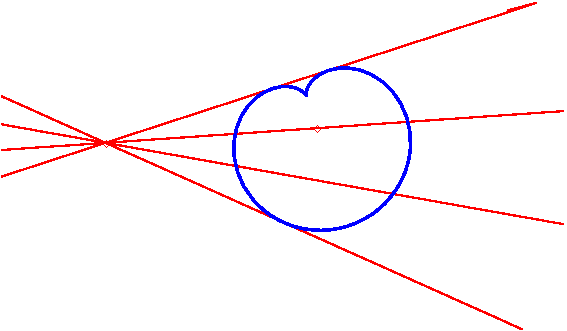
\includegraphics{Etrisec_2.pdf}
  \caption{Cardio{\"\i}de tritangente}
  \label{fig:Etrisec_2}
\end{figure}

\subsubsection*{Partie IV : cardio{\"\i}des}
\begin{figure}[ht]
  \centering
  \input{Etrisec_5.pdf_t}
  \caption{Roulement sans glissement}
  \label{fig:Etrisec_5}
\end{figure}
Soit $\mathcal{C}$ le cercle de centre $O$ et de rayon 1. Pour tout $\theta \in ]-\pi, \pi[$, on d{\'e}finit
\begin{itemize}
  \item $C_\theta$ : le point d'affixe $c_\theta=2e^{i\theta}$.
  \item $\mathcal{E}_\theta$ : le cercle de centre $C_\theta$ et
  de rayon 1.
  \item $F(\theta)$ est le point de $\mathcal{E}_\theta$ tel que l'angle orient{\'e} $(\overrightarrow{C_\theta O},\overrightarrow{C_\theta F(\theta)})=\theta$.
  \item $f(\theta)$ est l'affixe de $F(\theta)$.
  \item $S$ est le point d'affixe $s=1$.
  \item $M$ est le point d'affixe $m=\frac{3}{2}$.
\end{itemize}
On peut considérer que $F(\theta)$ est un point d'un cercle de rayon $1$ qui roule sans glisser (fig \ref{fig:Etrisec_4}) sur le cercle $\mathcal C$. 
\begin{enumerate}
  \item Donner (sans justification) une construction g{\'e}om{\'e}trique de $F(\theta)$ {\`a}  partir de $C_\theta$ en faisant intervenir la m{\'e}diatrice de  $[O,C_\theta]$.
  \item Montrer que
  \[f(\theta)=2e^{i\theta}-e^{2i\theta}\]
  \item {\'E}tude de la courbe param{\'e}tr{\'e}e
    \begin{enumerate}
        \item Comment est obtenu $F(-\theta)$ {\`a} partir de $F(\theta)$?
        \item Pr{\'e}ciser $f(0)$, $f(\frac{\pi}{2})$, $f(\pi)$, $f(\frac{\pi}{3})$,$f(\frac{2\pi}{3})$
        \item Mettre $f(\theta)-s$ et $f'(\theta)$ sous forme trigonom{\'e}trique.
        \item Montrer qu'il existe un seul point stationnaire {\`a} pr{\'e}ciser. Quelle est la limite de la direction de la tangente en ce point ?
        \item {\'E}tudier les variations des coordonn{\'e}es de $F(\theta)$.
        \item Tracer le support de la courbe param{\'e}tr{\'e}e. Cette  courbe est appel{\'e}e \emph{cardio{\"\i}de de centre} $O$.
    \end{enumerate}
  \item On note $T$ le point d'intersection de la tangente en $F(\theta)$ avec la droite d'{\'e}quation
  $x=\frac{3}{2}$.

    \begin{enumerate}
        \item Montrer que
        \begin{eqnarray*}
        \cos 3x &=& \cos x (1- 4\sin^2 x)\\
        \sin 3x &=& \sin x (3- 4\sin^2 x)
        \end{eqnarray*}
        \item Calculer l'ordonn{\'e}es de $T$. On trouvera une expression tr{\`e}s simple en fonction de $\frac{\theta}{2}$.
        \item  Montrer l'{\'e}galit{\'e} suivante entre les angles orient{\'e}s : \[3(\overrightarrow{TM},\overrightarrow{TO})=(\overrightarrow{TM},\overrightarrow{TF(\theta)})\]
  Formuler une propri{\'e}t{\'e} relative au centre d'une cardio{\"\i}de inscrite dans un angle et bitangente {\`a} un c{\^o}t{\'e}.
\end{enumerate}

\end{enumerate}
